% LaTeX Präsentationsvorlage (2013) der TU Graz, rev12, 2013/01/31
% !TeX encoding = UTF-8
\documentclass{beamer}
% \documentclass[aspectratio=169]{beamer}
% \usetheme{tugraz2013}
% \usetheme[notes]{tugraz2013}
\usepackage{../common/beamerthemetugraz2013}
\usepackage{color}
\usepackage{multicol}
\usepackage{bbding}
\usepackage{wasysym}
\usepackage{hyperref}
\usepackage{siunitx}
\usepackage{caption}
% \usepackage{minted}

\usepackage{listings}
\usepackage{xcolor}

\definecolor{codegreen}{rgb}{0,0.6,0}
\definecolor{codegray}{rgb}{0.5,0.5,0.5}
\definecolor{codepurple}{rgb}{0.58,0,0.82}
\definecolor{backcolour}{rgb}{0.95,0.95,0.92}
\lstdefinestyle{mystyle}{
    backgroundcolor=\color{backcolour},   
    commentstyle=\color{codegreen},
    keywordstyle=\color{magenta},
    numberstyle=\tiny\color{codegray},
    stringstyle=\color{codepurple},
    basicstyle=\ttfamily\footnotesize,
    breakatwhitespace=false,         
    breaklines=true,                 
    captionpos=b,                    
    keepspaces=true,                 
    numbers=left,                    
    numbersep=5pt,                  
    showspaces=false,                
    showstringspaces=false,
    showtabs=false,                  
    tabsize=2
}

\lstset{style=mystyle}

\usepackage{picture}
\usepackage{rotating}
\definecolor{darkred}{rgb}{0.85,0.16,0.0}
\definecolor{darkgreen}{rgb}{0.16,0.70,0.27}

\usepackage{xcolor}


\newcommand{\hrefu}[2]{\underline{\href{#1}{#2}}}
\newcommand{\hyperlinku}[2]{\underline{\hyperlink{#1}{#2}}}
\newcommand{\smallurl}[1]{%
  \begin{flushleft}
    \tiny\url{#1}
  \end{flushleft}
}
\newcommand{\smalltext}[1]{%
  \begin{flushleft}
    \tiny{#1}
  \end{flushleft}
}
\newcommand{\red}[1]{{\color{red} #1}}
\newcommand{\blue}[1]{{\color{blue} #1}}
\newcommand{\darkgreen}[1]{\textcolor{darkgreen}{#1}}
\newcommand{\darkred}[1]{\textcolor{darkred}{#1}}

\newcommand*{\vpointer}{\vcenter{\hbox{\scalebox{1.5}{\large\pointer}}}}

\newcommand{\be}[1]{\begin{equation} \label{#1}}
\newcommand{\ee}{\end{equation}}
\newcommand{\bea}[1]{\begin{eqnarray} \label{#1}}
\newcommand{\eea}{\end{eqnarray}}
\newcommand{\bean}{\begin{eqnarray*}}
\newcommand{\eean}{\end{eqnarray*}}

\newcommand{\non}{\nonumber\\}
\newcommand{\eq}[1]{(\ref{#1})}
\newcommand{\difp}[2]{\frac{\partial #1}{\partial #2}}
\newcommand{\br}{{\bf r}}
\newcommand{\bR}{{\bf R}}
\newcommand{\bA}{{\bf A}}
\newcommand{\bB}{{\bf B}}
\newcommand{\bE}{{\bf E}}
\newcommand{\bm}{{\bf m}}
%\renewcommand{\bm}{{\bf m}}
\newcommand{\bn}{{\bf n}}
\newcommand{\bN}{{\bf N}}
\newcommand{\bp}{{\bf p}}
\newcommand{\bP}{{\bf P}}
\newcommand{\bF}{{\bf F}}
\newcommand{\by}{{\bf y}}
\newcommand{\bz}{{\bf z}}
\newcommand{\bZ}{{\bf Z}}
\newcommand{\bV}{{\bf V}}
\newcommand{\bv}{{\bf v}}
\newcommand{\bu}{{\bf u}}
\newcommand{\bx}{{\bf x}}
\newcommand{\bX}{{\bf X}}
\newcommand{\bW}{{\bf W}}
\newcommand{\bJ}{{\bf J}}
\newcommand{\bj}{{\bf j}}
\newcommand{\bk}{{\bf k}}
\newcommand{\bTheta}{{\bf \Theta}}
\newcommand{\btheta}{{\boldsymbol\theta}}
\newcommand{\bOmega}{{\bf \Omega}}
\newcommand{\bomega}{{\boldsymbol\omega}}
\newcommand{\brho}{{\boldsymbol\rho}}
\newcommand{\rd}{{\rm d}}
\newcommand{\rJ}{{\rm J}}
\newcommand{\ph}{{\varphi}}
\newcommand{\te}{\theta}
\newcommand{\tht}{\vartheta}
\newcommand{\vpar}{v_\parallel}
\newcommand{\vparkb}{v_{\parallel k b}}
\newcommand{\vparkm}{v_{\parallel k m}}
\newcommand{\Jpar}{J_\parallel}
\newcommand{\ppar}{p_\parallel}
\newcommand{\Bpstar}{B_\parallel^*}
\newcommand{\intpi}{\int\limits_{0}^{2\pi}}
\newcommand{\summ}{\sum \limits_{m=-\infty}^\infty}
\newcommand{\tb}{\tau_b(\uv)}
\newcommand{\bh}{{\bf h}}
\newcommand{\cE}{{\cal E}}
\newcommand{\bsigma}{{\boldsymbol\sigma}}
\newcommand{\bS}{{\mathbf S}}
\newcommand{\bI}{{\mathbf I}}
\newcommand{\odtwo}[2]{\frac{\rd #1}{\rd #2}}
\newcommand{\pdone}[1]{\frac{\partial}{\partial #1}}
\newcommand{\pdtwo}[2]{\frac{\partial #1}{\partial #2}}
\newcommand{\ds}{\displaystyle} % commands


%% Titelblatt-Einstellungen
\title[]
{Python 12}
\author[E.~Wachmann]{\scriptsize Elias Wachmann
}
\date{2024} % \today für heutiges Datum verwenden
\institute[Institute of Theoretical and Computational Physics]
{
}
\instituteurl{www.tugraz.at}
% \institutelogo{kurz.pdf}
%~ \additionallogo{merged_logos}
\AtBeginSection[]{
  \begin{frame}
  \vfill
  \centering
  \begin{beamercolorbox}[sep=8pt,center,shadow=true,rounded=true]{title}
    \usebeamerfont{title}\insertsectionhead\par%
  \end{beamercolorbox}
  \vfill
  \end{frame}
}
\lstset{
    literate={Ö}{{\"O}}1
             {Ä}{{\"A}}1
             {Ü}{{\"U}}1
             {ß}{{\ss}}1
             {ü}{{\"u}}1
             {ä}{{\"a}}1
             {ö}{{\"o}}1
}

%%%%%%%%%%%%%%%%%%%%%%%%%%%%%%%%%%%%%%%%%%%%%%%%%%%%%%%%%%%%%%%%%%%%%%%%%%%%
\begin{document}
%%%%%%%%%%%%%%%%%%%%%%%%%%%%%%%%%%%%%%%%%%%%%%%%%%%%%%%%%%%%%%%%%%%%%%%%%%%%
\titleframe

\section*{Content}

\begin{frame}
\frametitle{Content}
  \tableofcontents
\end{frame}
\section{What is object oriented programming?}
\begin{frame}
  \frametitle{Intro to object oriented programming}
  How do we classify things in the real world?\\
  \vspace{5mm}
  We group them by their properties and their behaviour.\\
  \vspace{5mm}
  An \textbf{object} like a planet is can be described by its properties like mass, radius, position, velocity, etc.\\
  \vspace{5mm}
  We can also describe its behaviour like how it moves around the sun.\\
\end{frame}
\begin{frame}
  \frametitle{What are classes?}
  \textbf{Classes} are a way to abstract real world things into categories.\\
  \begin{minipage}[t]{0.55\textwidth}
    \vspace{-3cm}
    Not all planets are the same, but they can be described by the same properties and behaviour.\\
    We can use a \textbf{class} that describes the properties and behaviour of a planet (an \textbf{object}).\\
  \end{minipage}%
  \hspace{5mm}
  \begin{minipage}[t]{0.35\textwidth}
    \centering
    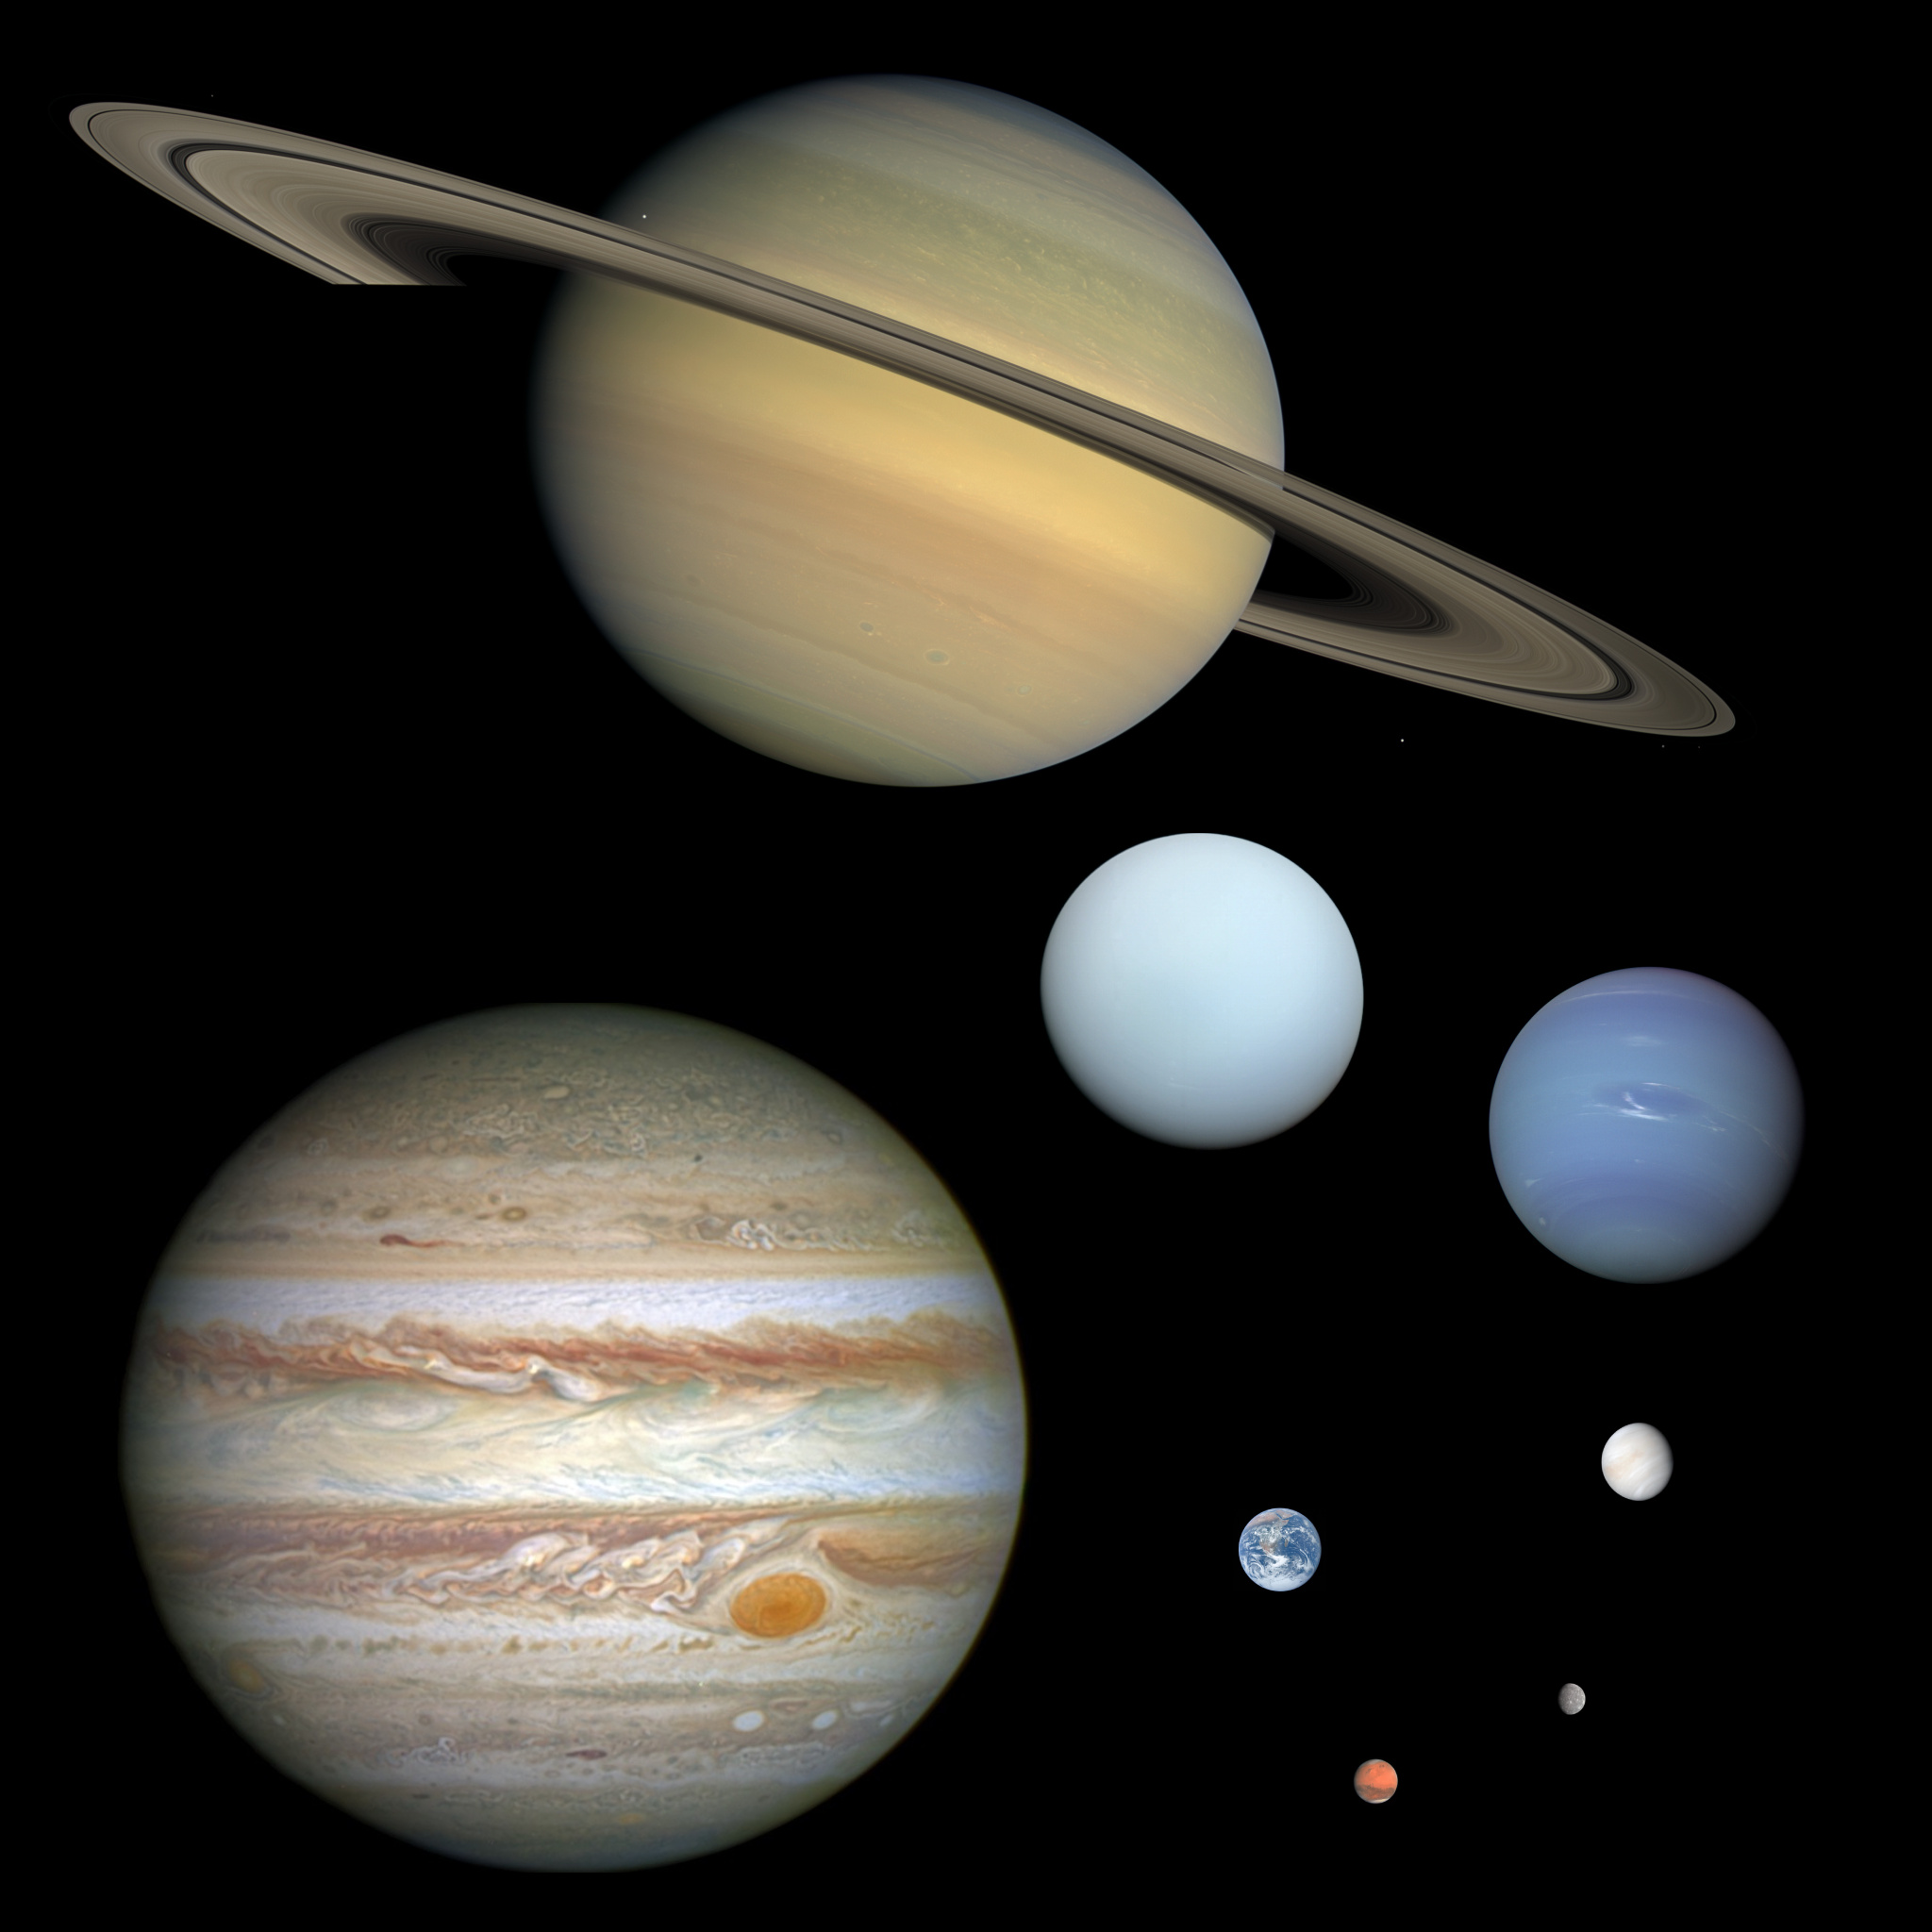
\includegraphics[width=0.9\textwidth]{fig/Planet_collage_to_scale.jpg}
    \smallurl{https://upload.wikimedia.org/wikipedia/commons/c/cf/Planet_collage_to_scale.jpg}
\end{minipage}
\end{frame} 
\begin{frame}
  \frametitle{Describe objects within a class}
  How can we distinguish between different planets now?\\
  \vspace{5mm}
  \textbf{Earth}: m = \SI{5.97e24}{kg}, r = 6371 km, \dots\\
  \vspace{5mm}
  \textbf{Mars}: m = \SI{6.41e23}{kg}, r = 3389.5 km, \dots\\
  \vspace{5mm}
  \textbf{Jupiter}: m = \SI{1.90e27}{kg}, r = 69911 km, \dots\\
\end{frame}
\section{Python classes}
\begin{frame}
  \frametitle{Let's define a Planet class}
  In python we can define a class like this:\\
  \lstinputlisting[language=python, lastline=5]{examples/planets.py}
  \vspace{5mm}
  The \textbf{\hrefu{https://docs.python.org/3/tutorial/classes.html}{class}}-keyword tells python that we want to define a class.\\
\end{frame}
\begin{frame}
  \frametitle{What is the \_\_init\_\_ function?}
  The \textbf{\hrefu{https://docs.python.org/3/reference/datamodel.html\#object.__init__}{\_\_init\_\_}} function is called when we create a new object of the class.\\
  \vspace{5mm}
  Objects are therefore concrete \textbf{instances} of a class.\\
  \vspace{5mm}
  In our example the Planet class takes the arguments \textbf{mass} and \textbf{radius} and stores them as \textbf{attributes} of the object.\\
  \vspace{5mm}
  How can we access these attributes and what is the \textbf{\hrefu{https://docs.python.org/3/faq/programming.html\#what-is-self}{self}}-keyword?\\
\end{frame}
\begin{frame}
  \frametitle{Pythons self keyword}
  The \textbf{self} keyword is a reference to the object itself.\\
  \lstinputlisting[language=python,firstline=2, lastline=5]{examples/planets.py}
  This means: If you want to create an attribute of a class, you simply write \texttt{\textbf{self}.variable\_name}
  \vspace{5mm}
  \textbf{self} also has to be passed in as the first argument to every function defined inside the class! 
\end{frame}
\begin{frame}
  \frametitle{Methods -- class functions}
  \textbf{\hrefu{https://docs.python.org/3/tutorial/classes.html\#methods}{Methods}} are functions inside a class. They can only be accessed by objects of that class and \textbf{self} is their first argument.  
  \lstinputlisting[language=python, lastline=8]{examples/planets.py}
\end{frame}
\begin{frame}
  \frametitle{Let's create a Planet}
  Finally let's create a planet object: 
  \lstinputlisting[language=python, firstline=13, lastline=14]{examples/planets.py}
  Just pass in the initial arguments just like you would for functions. 
  \lstinputlisting[language=python, firstline=15, lastline=16]{examples/planets.py}
  We can now call our defined class method on objects. 
\end{frame}
\begin{frame}
  \frametitle{Modify objects}
  Certainly a method can modify attributes of an object like in the following example the name. 
  \lstinputlisting[language=python, firstline=10, lastline=12]{examples/planets.py}  

  \lstinputlisting[language=python, firstline=17]{examples/planets.py}  
  This only changes the name of the \glq earth\grq-object while the \glq mars\grq-object is not affected. 
\end{frame}
%%%%%%%%%%%%%%%%%%%%%%%%%%%%%%%%%%%%%%%%%%%%%%%%%%%%%%%%%%%%%%%%%%%%%%%%%%%%
\section{Dunder-methods}
\begin{frame}
  \frametitle{Dunder-methods}
  \textbf{\hrefu{https://docs.python.org/3/reference/datamodel.html\#special-method-names}{Dunder-methods}} are special methods that are called by python in certain situations.\\
  \vspace{5mm}
  We have seen the \textbf{\hrefu{https://docs.python.org/3/reference/datamodel.html\#object.__init__}{\_\_init\_\_}} method, which is called when a new object is created, before.\\
  Further examples include: 
  \begin{itemize}
    \item \textbf{\hrefu{https://docs.python.org/3/reference/datamodel.html}{\_\_str\_\_}} method is called when we try to convert an object to a string.\\
    \item \textbf{\hrefu{https://docs.python.org/3/reference/datamodel.html}{\_\_add\_\_}} method is called for + operator.\\
    \item  \textbf{\hrefu{https://docs.python.org/3/reference/datamodel.html}{\_\_lt\_\_, \_\_le\_\_, \_\_eq\_\_, \_\_ne\_\_, \_\_gt\_\_, \_\_ge\_\_}} methods used for comparisons. 
  \end{itemize}
\end{frame}
\begin{frame}
  \frametitle{Dunder-methods -- Examples}
  One can now implement dunder methods for our custom classes to make certain functionality (like comparisons between objects) possible.\\
  \lstinputlisting[language=python, firstline=13, lastline=19]{examples/planets\_dunder.py}
\end{frame}
\begin{frame}
  \frametitle{Dunder-methods -- Iterators}
  \textbf{\hrefu{https://docs.python.org/3/reference/datamodel.html\#object.__iter__}{\_\_iter\_\_}} and \textbf{\hrefu{https://docs.python.org/3/reference/datamodel.html\#object.__next__}{\_\_next\_\_}} are special methods that allow us to iterate over objects.\\
  \vspace{5mm}
  While \textbf{\_\_iter\_\_} returns an iterator object, \textbf{\_\_next\_\_} returns the next element of the iterator.\\
  \vspace{5mm}
  This allows us to specify what a while/for loop should do when it encounters an object of our class.\\
\end{frame}
\begin{frame}
  \frametitle{Dunder-methods -- Iterators -- Example}
  Let's define a new class: 
  \lstinputlisting[language=python, lastline=8]{examples/iter.py}
  \dots
\end{frame}
\begin{frame}
  \frametitle{Dunder-methods -- Iterators -- Example}
  \vspace{-10mm}
  \lstinputlisting[language=python, firstline=11, lastline=22]{examples/iter.py}
  \dots
\end{frame}
\begin{frame}
  \frametitle{Dunder-methods -- Iterators -- Example}
  \vspace{-10mm}
  \lstinputlisting[language=python, firstline=24]{examples/iter.py}
\end{frame}
%%%%%%%%%%%%%%%%%%%%%%%%%%%%%%%%%%%%%%%%%%%%%%%%%%%%%%%%%%%%%%%%%%%%%%%%%%%%
\section{Inheritance}
\begin{frame}
  \frametitle{Inheritance}
  Inheritance is a way to create a new class from an existing class.\\
  \vspace{5mm}
  The new class is called \textbf{child class} and the existing class is called \textbf{parent class}.\\
  \vspace{5mm}
  The child class inherits all attributes and methods from the parent class and may expand on them or overwrite them.\\
\end{frame}
\begin{frame}
  \frametitle{Inheritance}
  We can create a child class by passing the parent class as an argument to the child class definition: 
  \lstinputlisting[language=python, firstline=20, lastline=20]{examples/inheritance.py}
  Here the \textbf{child class} Dog is instantiated with the \textbf{parent class} Animal as an argument.\\
  \lstinputlisting[language=python, firstline=1, lastline=5]{examples/inheritance.py}
  Animal implements a \textbf{\_\_str\_\_} method like seen before.\\
\end{frame}
\begin{frame}
  \frametitle{Inheritance -- super method}
  The \textbf{\hrefu{https://docs.python.org/3/library/functions.html\#super}{super}} method allows us to call methods of the parent class.\\
  \vspace{5mm}
  This way we can call \textbf{\_\_init\_\_} in the parent class from the child class: \\
  \lstinputlisting[language=python, firstline=13, lastline=14]{examples/inheritance.py}
\end{frame}
\begin{frame}
  \frametitle{Inheritance -- Example}
  \vspace{-10mm}
  \lstinputlisting[language=python, firstline=13, lastline=25]{examples/inheritance.py}
\dots
\end{frame}
\begin{frame}
  \frametitle{Inheritance -- Example}
  \vspace{-10mm}
  \lstinputlisting[language=python, firstline=27, lastline=31]{examples/inheritance.py}
  Now the method \textbf{make\_sound} is implemented in both children classes.\\
  \vspace{5mm} 
  Cats make a \textbf{meow} sound while dogs make a \textbf{woof} sound.\\
\end{frame}
\begin{frame}
  \frametitle{Inheritance -- Overwriting methods}
  Ok let's add another child class, a frog: 
  \lstinputlisting[language=python, firstline=32, lastline=34]{examples/inheritance.py}
  We should also add a \textbf{make\_sound} method to the parent class:
  \lstinputlisting[language=python, firstline=7, lastline=8]{examples/inheritance.py}
\end{frame}
\begin{frame}
  \frametitle{Inheritance -- Overwriting methods}
  If we now instantiate a frog and call \textbf{make\_sound} we get:
  \lstinputlisting[language=python, firstline=35, lastline=36]{examples/inheritance.py}
  \vspace{5mm}
  Because there is no \textbf{make\_sound} method in the frog class, the method from the parent class is used.\\
  \vspace{5mm}
  The Cat and Dog class \textbf{overwrite} the method from the parent class and use their own implementation.\\
\end{frame}

\section{Wrap up + What's next?}
\begin{frame}
  \frametitle{Wrap up}
  By now you should have a good understanding of the basics of python programming for scientific computing.\\
  \vspace{5mm}
  You have learned how to use python to: 
  \begin{itemize}
    \item import data
    \item modify and analyse the data
    \item plot/visualize the data
    \item write your own functions
    \item define classes and objects \dots
  \end{itemize}
\end{frame}
\begin{frame}
  \frametitle{What's next?}
  There are many more topics to cover in (python) programming \dots\\
  \vspace{5mm}
  Next up: Computational Physics in 5th semester!\\
  \begin{itemize}
    \item numerical methods for solving differential equations
    \item methods for solving linear systems
    \item solving partial differential equations
    \item efficient eigenvalues of matrices / compression
  \end{itemize}
\end{frame}
\begin{frame}
  \frametitle{What's next?}
  Other courses you might be interested in:
  \begin{itemize}
    \item Einführung in die strukturierte Programmierung (C) [INB.04000UF, 
    INB.05000UF]
    \item Objektorientierte Programmierung 1 (C++) [INF.07002UF, INF.08008UF]
    \item Data Management (SQL) [INF.01017UF, INF.02018UF]
    \item Datenstrukturen und Algorithmen 1 [INF.04032UF, INF.03031UF]
    \item Software Engineering in Physics [PHT.528UF]
    \item \dots
  \end{itemize}
\end{frame}
\end{document}
%%%%%%%%%%%%%%%%%%%%%%%%%%%%%%%%%%%%%%%%%%%%%%%%%%%%%%%%%%%%%%%%%%%%%%%%%%%%

%% EOF
